\documentclass[11pt,a4paper]{article}

% ----------------------------------------------------------------------
% Packages
% ----------------------------------------------------------------------
\usepackage[utf8]{inputenc}
\usepackage[T1]{fontenc}
\usepackage[margin=2.2cm,top=2cm,bottom=2.3cm]{geometry}
\usepackage{graphicx}
\usepackage{textcomp}
\usepackage[colorlinks=true,linkcolor=black,urlcolor=blue,citecolor=black]{hyperref}
\usepackage{fancyhdr}
\usepackage{lastpage}
\usepackage{tikz}
\usepackage{enumitem}
\usepackage{needspace}
\usepackage{datetime2}


% ----------------------------------------------------------------------
% Page layout
% ----------------------------------------------------------------------
\setlength{\parindent}{0pt}
\setlength{\parskip}{0pt}

\pagestyle{fancy}
\fancyhf{}
\fancyfoot[R]{\footnotesize Page \thepage{} of \pageref{LastPage}}
\renewcommand{\headrulewidth}{0pt}
\renewcommand{\footrulewidth}{0pt}

% ----------------------------------------------------------------------
% Custom commands
% ----------------------------------------------------------------------

% Section heading with a horizontal rule underneath
\newcommand{\cvsection}[1]{%
  \vspace{15pt}%
  \noindent{\Large #1}\par%
  \vspace{-7pt}%
  \noindent\rule{\linewidth}{0.6pt}\par%
  \vspace{10pt}%
}

% A CV entry: a date / label on the left, content on the right
\newcommand{\cvitem}[2]{%
  \noindent\begin{minipage}[t]{0.19\linewidth}%
    \textit{#1}%
  \end{minipage}%
  \begin{minipage}[t]{0.79\linewidth}%
    \raggedright#2%
  \end{minipage}\par%
  \vspace{7pt}%
}

% A publication / working paper entry (hanging indent, no date column)
\newcommand{\pubitem}[1]{%
  \Needspace{6\baselineskip}%
  \par\noindent\hangindent=1.2em\hangafter=1 #1\par%
  \vspace{6pt}%
}

% Skill level indicator: filled vs. open circles, n out of 5
\newcommand{\skilllevel}[1]{%
  \foreach \i in {1,...,5}{%
    \ifnum\i>#1
      \tikz[baseline=-0.55ex]{\draw[gray,line width=0.6pt] (0,0) circle (1.4pt);}%
    \else
      \tikz[baseline=-0.55ex]{\fill[black] (0,0) circle (1.4pt);}%
    \fi
    \hspace{1pt}%
  }%
}

% A row in the skills table
\newcommand{\skillrow}[2]{#1 & \skilllevel{#2} \\}

% For comments
\newcommand{\co}[1]{{\color{red}\textbf{[}#1\textbf{]}}}

\begin{document}

% ========================================================================
% Header
% ========================================================================
\noindent
\begin{minipage}[b]{0.78\textwidth}
  {\fontsize{28}{32}\selectfont Christian Vedel}\\[2pt]
  \rule{\linewidth}{0.8pt}\\[8pt]
  \textit{Updated: \DTMtoday}\\[8pt]
  Historical Economics and Development Group (HEDG)\\
  Department of Economics\\
  University of Southern Denmark\\[8pt]
  Email: \href{mailto:christian-vs@sam.sdu.dk}{christian-vs@sam.sdu.dk}\\
  Languages: Fluent: Danish, English; \quad Basic: Norwegian, Swedish
\end{minipage}%
\hfill
\begin{minipage}[b]{0.22\textwidth}
  \raggedleft
  \setlength{\fboxsep}{0pt}
  \setlength{\fboxrule}{1pt}
  \fbox{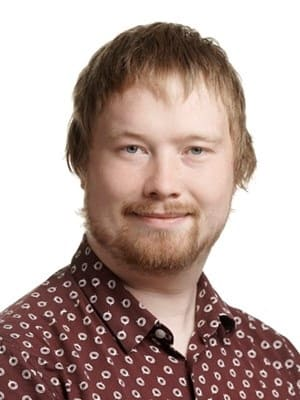
\includegraphics[width=\linewidth]{photo.jpg}}
\end{minipage}

\vspace{10pt}

{\footnotesize\textit{A note on my last name: I currently share my last name `Sørensen' with 101,473 other Danes. For this reason, it is not of much use as an identifier in a population of only 5.8 mil. Instead, I use my middle name: `Vedel', which I share with fewer people.}}


% CV main body begins here
\cvsection{Research interests}
What drives all of my research is a simple premise: much of what we know about the economic cosmos is limited by what we can measure. I build machine learning tools and large-scale historical datasets to recover economic measurements from the past, and combine them with causal inference methods to study how geography and institutions shape prosperity. The ultimate aim is to use the vastness of history to give policy makers better maps of what can be changed, what cannot, and where the limits of policy lie.
\\ \\
\textbf{Keywords:} Economic history, Economic Development, Causal Inference, Machine Learning, Economic Geography, Large-Scale Historical Data

\cvsection{Academic positions}
\cvitem{2023--2027}{%
  Assistant Professor\\
  \textit{Fixed-term, non-tenure-track appointment}\\
  \textit{Department of Economics, \\Historical Economics and Development Group (HEDG)}\\
  \textit{University of Southern Denmark}%
}

\cvitem{2024--present}{%
  External Lecturer\\
  \textit{Summer School in European Economic History}\\
  \textit{Department of Economics, University of Copenhagen}%
}

\cvitem{2018--2019}{%
  Student Research Assistant\\
  \textit{Department of Economics, University of Southern Denmark}%
}

\cvitem{2017}{%
  Teaching Assistant \\
  \textit{Department of Economics, University of Southern Denmark}%
}

\cvsection{Education}
\cvitem{2020--2023}{%
  PhD in Economics,\\
  University of Southern Denmark\\
  \underline{Title:} \textit{Natural Experiments in Geography and Institutions:
  Essays in the Economic History of Denmark}\\
  \underline{Main advisor:} Paul Sharp\\
  \underline{Co-advisors:} Christian Møller Dahl, Casper Worm Hansen%
}

\cvitem{2022}{%
  Visiting Research Student, (Jan. 17 -- May 31)\\
  Department of Economic History, London School of Economics\\
  \underline{Host:} Prof. Max Schulze%
}

\cvitem{2015--2021}{%
  BSc and MSc in Economics,\\
  University of Southern Denmark%
}

\cvitem{2010--2013}{%
  International Baccalaureate Diploma Programme (IBDP),\\
  Nyborg Gymnasium%
}

\cvsection{Funding \& Prizes}
\cvitem{2027--2030}{%
  \textbf{Danish Independent Research Fund}, DFF-Forskningsprojekt2:
  6\,114\,741 DKK\\
  \textit{Denmark's Path to Economic Development: Structural Transformation,
  Free-Market Trade, and Migration from 1790 to Today}\\
  PI: Casper Worm Hansen. Named project participant%
}

\cvitem{2023}{%
  \textbf{EHS Best New Researcher Prize}\\
  \textit{Awarded at the Economic History Society's Annual Conference}%
}

\cvitem{2022}{%
  \textbf{Augustinusfonden}: 15\,000 DKK (\texteuro{}2\,016)\\
  \textit{Towards research stay at the London School of Economics}%
}

\cvsection{Publications}
\pubitem{Bentzen, J. S., Boberg-Fazlić, N., Sharp, P., Skovsgaard, C. V., \& Vedel, C. (2026). Holy cows and spilled milk: The impact of religious missions on firm-level productivity. \textit{Journal of Development Economics}, 179, 103651. \href{https://doi.org/10.1016/j.jdeveco.2025.103651}{doi.org/10.1016/j.jdeveco.2025.103651}}

\pubitem{McLaughlin, E., Sharp, P., Tsoukli, X., \& Vedel, C. (2026). Ireland in a Danish mirror: A microlevel comparison of the productivity of Danish and Irish creameries before the First World War. \textit{Business History}, 68(3), 596--612. \href{https://doi.org/10.1080/00076791.2025.2486643}{doi.org/10.1080/00076791.2025.2486643}}

\pubitem{Henriques, S. T., Sharp, P., Tsoukli, X., \& Vedel, C. (2024). Adaptability, diversification, and energy shocks: A firm level productivity analysis. \textit{Energy Economics}, 139, 107887. \href{https://doi.org/10.1016/j.eneco.2024.107887}{DOI}}

\pubitem{Sharp, P., S. Henriques, E. McLaughlin, X. Tsoukli, and C. Vedel (2023). A Microlevel Analysis of Danish Dairy Cooperatives: Opportunities for Large Data in Business History. \textit{Enterprise \& Society}, 1--29. \href{https://doi.org/10.1017/eso.2023.5}{doi.org/10.1017/eso.2023.5}}

\pubitem{McLaughlin, E., P. Sharp, X. Tsoukli, and C. Vedel (2023). A Firm Level Database of Irish Creameries, 1897--1921. \textit{Irish Economic and Social History}. \href{https://doi.org/10.1177/03324893231161927}{doi.org/10.1177/03324893231161927}}

\cvsection{Working papers}
\pubitem{Vedel, C. (2024; latest version 2026). A Perfect Storm: First-Nature Geography and Economic Development. Job market paper; EHES Working Paper 262. \href{https://arxiv.org/abs/2408.00885}{arxiv.org/abs/2408.00885}. \textit{Winner of the Economic History Society's 2023 New Researcher Prize.} \textbf{Job Market Paper}}

\pubitem{Johansen, T., Koschnick, J., \& Vedel, C. (2026). How to deal with machine learning bias in economic history. \href{https://arxiv.org/abs/2606.28063}{arxiv.org/abs/2606.28063}.}

\pubitem{Dahl, C. M., Johansen, T., \& Vedel, C. (2024; latest version 2026). Breaking the HISCO Barrier: Automatic Occupational Standardization with OccCANINE. EHES Working Paper 255. \href{https://arxiv.org/abs/2402.13604}{arxiv.org/abs/2402.13604}.}

\pubitem{G\"orges, T., Rove, M. {\O}., Sharp, P., \& Vedel, C. (2025; latest version 2025). Tracks to Modernity: Railroads, Growth, and Social Movements in Denmark. Revise and resubmit, \textit{European Review of Economic History}. \href{https://arxiv.org/abs/2502.21141}{arxiv.org/abs/2502.21141}.}

\pubitem{Aaskoven, L., \& Vedel, C. (2026). Physical Memories of the Past and Support for the Far-Right: Evidence from Inter-War Denmark. EHES Working Paper 295. \href{https://ehes.org/wp/EHES_295.pdf}{ehes.org/wp/EHES\_295.pdf}.}

\pubitem{McLaughlin, E., Sharp, P., Skovsgaard, C. V., \& Vedel, C. (2024). Milk Wars: Cooperation, Contestation, Conflict and the Irish War of Independence. EHES Working Paper 272. \\ \href{https://www.ehes.org/wp/EHES_272.pdf}{ehes.org/wp/EHES\_272.pdf}.}

\pubitem{Bentzen, J. S., Boberg-Fazlić, N., Sharp, P., Skovsgaard, C. V., \& Vedel, C. (2024). Assimilate for God: The Impact of Religious Divisions on Danish American Communities. EHES Working Paper 253. \href{https://www.ehes.org/wp/EHES_253.pdf}{ehes.org/wp/EHES\_253.pdf}.}


\cvsection{Other publications}
\pubitem{Vedel, C. (2023). Natural Experiments in Geography and Institutions: Essays in the Economic History of Denmark. [Ph.D. thesis, SDU]. Syddansk Universitet. Det Samfundsvidenskabelige Fakultet. \href{https://doi.org/10.21996/jt34-zc23}{doi.org/10.21996/jt34-zc23}}

\pubitem{Vedel, C. (2025). Review of \textit{Danish Capitalism in the 20th Century: A Business History of an Innovistic Mixed Economy}, by Stefan Kirkegaard Sl{\o}k-Madsen. \textit{Scandinavian Economic History Review}, 73(2), 160--162.}

\pubitem{Vedel, C. (2022). Trap Denmark: Tønder, Aabenraa, Sønderborg (vol 17). \textit{Scandinavian Economic History Review}. \href{https://doi.org/10.1080/03585522.2021.2013315}{doi.org/10.1080/03585522.2021.2013315}}

\pubitem{Vedel, C. (2022). A very natural experiment: using nature to measure how infrastructure produces growth. London School of Economics, Economic History Blog. \href{https://blogs.lse.ac.uk/economichistory/2022/05/26/a-very-natural-experiment-using-nature-to-measure-how-infrastructure-produces-growth/}{blogs.lse.ac.uk/economichistory (2022)}}

\cvsection{Teaching experience}
\noindent\textit{S: Spring semester; F: Fall semester}

\vspace{6pt}

\cvitem{2026S}{%
  \textbf{Statistics}\\
  Course coordinator and lecturer. Introductory statistics for undergraduate Economics students \\
  Find open source teaching material here: \href{https://github.com/christianvedels/Introductory_statistics}{github.com/christianvedels/Introductory\_statistics}
}

\cvitem{2024--2026}{%
  \textbf{The Economic History of Europe}\\
  \textit{Summer school}\\
  University of Copenhagen%
}

\cvitem{2024-2026}{
    \textbf{Historical Perspectives on Current Economics Issues: Big Data and Applications}\\
    \textit{HEDG PhD Summer School}\\
    \textit{Teaching a two lecture module on Machine Learning for Economic History together with Torben Johansen}
    Slides: \href{https://github.com/TorbenSDJohansen/hedg-summer-school}{github.com/TorbenSDJohansen/hedg-summer-school}
}

\cvitem{2023F--2025F}{%
  \textbf{News and Market Sentiment Analysis}\\
  Lecturer. Course on natural language processing for students in the Data Science Masters programme. Find open source course material here: \href{https://github.com/christianvedels/News_and_Market_Sentiment_Analytics}{github.com/christianvedels/News\_and\_Market\_Sentiment\_Analytics}%
}



\cvitem{2025S}{%
  \textbf{Statistics}\\
  Lecturer. Introductory statistics for undergraduate Business Administration and European Studies students%
}

\cvitem{2023F--2024S}{%
  \textbf{Microeconomics}\\
  Lecturer. Introductory microeconomics for business students%
}

\cvitem{2022F}{%
  \textbf{Business History}\\
  Lecturer with Elena Korchmina%
}

\cvitem{2020--2022}{%
  \textbf{Tietgen talent track}\\
  Talent track for high school students from Tietgen business high school. I coordinate the program and teach everything from basic economic theory to latest research and basic statistics%
}

\cvitem{2020F}{%
  \textbf{Introduction to Business and Economic History (undergraduate)}\\
  Teaching assistant (partly online due to COVID).%
}

\cvitem{2020--2021}{%
  \textbf{Regression Analysis (undergraduate)}\\
  Guest lecture for one week both years. Taught introduction to the R statistical programming language.%
}

\cvitem{2020S}{%
  \textbf{Econometrics II (undergraduate)}\\
  Teaching assistant (partly online due to COVID)%
}

\cvitem{2017F}{%
  \textbf{Macroeconomics (undergraduate)}\\
  Teaching assistant%
}

\cvsection{Supervision}

\textbf{PhD students} \\
\cvitem{2024--2027}{Co-supervisor of PhD student Maret Anne Grapengeter (University of Oslo)}

\textbf{Master thesis students (Economics)} \\
\cvitem{2025}{Lea Lundberg Yssing, Sharmin Ather Keya}

\textbf{Master thesis students (Mathematical Economics)} \\
\cvitem{2026}{Katrine Enghoff Olsen, Lajza Prekazi} 

\textbf{Master thesis students (Data Science)} \\
\cvitem{2026}{Frederikke Buchsti Hermansen, Christoffer Johan Meilby Nobel, Rune Dissing Bjerring}
\cvitem{2025}{Lukas Rask Svendsen}

\cvsection{Presentations}
\cvitem{2026}{%
  Social Science History Association, SSHA (Atlanta); Danish Society for Economic and Social History (SDU); Workshop: Computational Economic History (CSH Vienna); Workshop: Big Data and Machine Learning in Economic History (Uppsala); Economic History Society Centenary Conference (London); CEPR Workshop (University of Copenhagen); Public Lecture for the Society of Transport Economics (Copenhagen)    
}

\cvitem{2025}{%
  Social Science History Association (Chicago); Applied Economic Seminar Series (UCPH); LEAP Workshop on Economic History in the Age of AI (Stellenbosch); Swedish Economic History Meeting and Scandinavian Society for Economic and Social History Conference (Ume{\aa}); European Network for the Comparative History of Population Geography and Occupational Structure (Cracow); European Society of Historical Demography Conference (Bologna)%
}

\cvitem{2024}{%
  2\textsuperscript{nd} Norwegian Winter Games (Oslo); Workshop on Machine Learning at the Department of Economic History (Lund); 13\textsuperscript{th} Annual Growth Workshop, HEDG (Odense); Economic History Society Annual Conference (Newcastle); 3\textsuperscript{rd} Danish Historical Political Economy Workshop (Odense); CITP conference (Nottingham); Advanced Methods Workshop (Lyon); Annual Meeting of the Danish Econometrics Society (Sandbjerg)%
}

\cvitem{2023}{%
  Seminar at the Department of Economic History (Lund); 12\textsuperscript{th} Annual Growth Workshop, HEDG (Odense); Economic History Society annual conference (Warwick); PhD seminar at the Department of Economics (Odense); End of semester workshop at the Department of Economic (Copenhagen); 9\textsuperscript{th} World Cliometrics Conference; 4\textsuperscript{th} Annual Conference of the Scandinavian Society for Economic and Social History (Lund); ENCHOS Conference (Linz); 9\textsuperscript{th} Annual Meeting of the Danish Society of Economic and Social History (Copenhagen)%
}

\cvitem{2022}{%
  XIX World Economic History Congress (Paris); EHES conference 2022 (Gronningen); LSE Graduate Economic History Seminar (London); 11\textsuperscript{th} Annual Growth Workshop, HEDG (Odense); 3\textsuperscript{rd} Scandinavian Meeting for Economic and Social History (Odense); HEDG Miniworkshop for young scholars (Odense)%
}

\cvitem{2021}{%
  Agricliometrics IV, UCIII Madrid; HEDG Miniworkshop for young scholars; DGPE Annual meeting; PhD seminar at the Department of Economics (SDU, Odense)%
}

\cvitem{2020}{%
  DGPE Annual meeting; PhD seminar at the Department of Economics (SDU, Odense)%
}

%\Needspace{10\baselineskip}
\cvsection{Academic service}
\cvitem{Refereeing}{%
  \textit{Review of Economics and Statistics};
  \textit{Scandinavian Economic History Review};
  \textit{Demographic Research};
  \textit{Digital Scholarship in the Humanities};
  \textit{Historical Methods}; \\
  \textit{Program Committee of International Conference on Natural Language and Speech Processing (ICNLSP)}
}

\cvitem{Community}{%
  Editor, EHES Working Paper Series, European Historical Economics Society\\
  Board member, Danish Society for Economic and Social History%
}

\cvitem{Organisation}{%
  Co-organiser, Annual Workshop on Growth, History and Development (HEDG) (many times)\\
  Co-organiser of Policy Event (2025, 2026)
}

\newpage
\cvsection{Non-academic employment}
\cvitem{2019--2020}{%
  \textbf{Number Crunch}, Odense\\
  My own small data consulting firm%
}

\cvitem{2018--2019}{%
  \textbf{Municipality of Copenhagen}, Copenhagen\\
  Student assistant in the department of data and analysis of the health and care administration%
}




\end{document}
